\subsection{Peak Baseline Fitting}

Peak fitting involves using the least-squares method in identifying and quantifying the baseline and peaks in the spectral data that correspond to specific soil components \cite{gardner_use_2011}. This method is useful for extracting information about the concentration of individual elements or compounds in the soil. For effective peak fitting, the data is filtered to focus on the peak area.

The fitting function is defined as:
\begin{equation}
F_f = F_p + F_b
\end{equation}

where $F_p$ is the peak function (e.g., Gaussian) and $F_b$ is the baseline function (e.g., linear or exponential falloff).

\begin{table}[H]
\centering
\caption{Function parameterizations for peak fitting}
\label{tab:functions}
\begin{tabular}{ll}
\toprule
Function Type & Example Expression \\
\midrule
Linear & $ax + b$ \\
Exp Falloff & $a \cdot \exp(-b \cdot x) + c$ \\
Gaussian & $a \cdot \exp(-((x - b)^2)/c^2) + d$ \\
\bottomrule
\end{tabular}
\end{table}

The baseline function is subtracted from the fitted function to isolate the peak, and the area under the peak is calculated to quantify the concentration of the corresponding element or compound in the soil.

\begin{figure}[H]
\centering
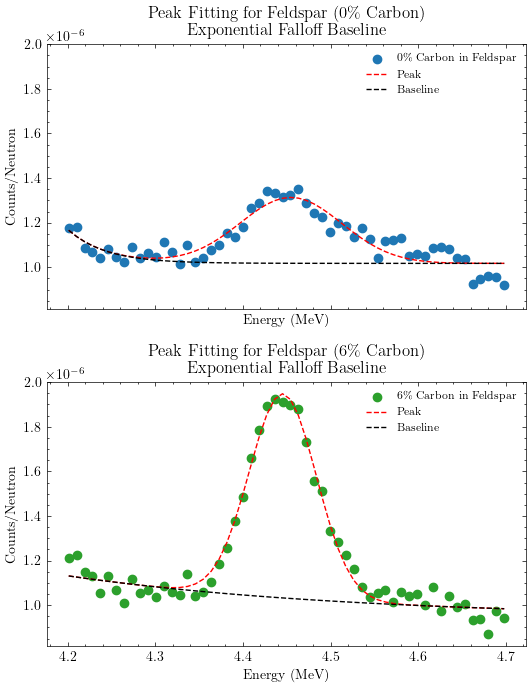
\includegraphics[width=0.8\textwidth]{../Figures/Analysis/peak_fitting_feldspar_subplots.png}
\caption{Peak fitting example showing fitted peak and baseline for feldspar spectrum}
\label{fig:peak_fitting}
\end{figure}

The final prediction is calibrated using the peak areas.

\begin{figure}[H]
\centering
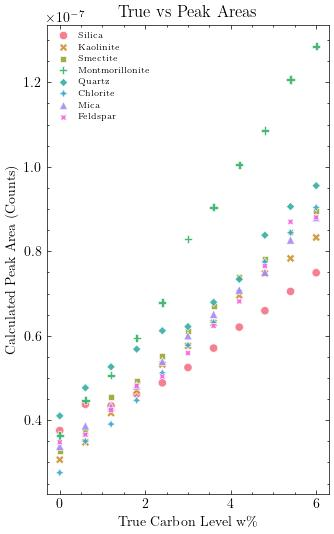
\includegraphics[width=0.8\textwidth]{../Figures/Analysis/carbon_level_vs_predicted_pf.jpg}
\caption{Peak fitting prediction results showing carbon level vs predicted values}
\label{fig:peak_predictions}
\end{figure}